\section{Εισαγωγή}
Ο κατακερματισμός (hashing) αποτελεί μια από τις βασικές τεχνικές στη επιστήμη των υπολογιστών. Χρησιμοποιείται στις δομές δεδομένων αλλά και σε άλλα πεδία της πληροφορικής όπως η κρυπτογραφία. Στο εργαστήριο αυτό θα παρουσιαστεί η δομή δεδομένων πίνακας κατακερματισμού χρησιμοποιώντας δύο διαδεδομένες υλοποιήσεις: την ανοικτή διευθυνσιοδότηση και την υλοποίηση με αλυσίδες. Επιπλέον, θα παρουσιαστούν δομές της STL όπως η unordered\_set και η unordered\_map οι οποίες στηρίζονται στην τεχνική του κατακερματισμού. Ο κώδικας όλων των παραδειγμάτων, όπως και στα προηγούμενα εργαστήρια, βρίσκεται στο \href{https://github.com/chgogos/ceteiep_dsa}{https://github.com/chgogos/ceteiep\_dsa}.

\section{Τι είναι ο κατακερματισμός;}
Ο κατακερματισμός είναι μια μέθοδος που επιτυγχάνει ταχύτατη αποθήκευση, αναζήτηση και διαγραφή δεδομένων. Σε ένα σύστημα κατακερματισμού τα δεδομένα αποθηκεύονται σε έναν πίνακα που ονομάζεται πίνακας κατακερματισμού (hash table). Θεωρώντας ότι τα δεδομένα είναι εγγραφές που αποτελούνται από ζεύγη τιμών της μορφής κλειδί-τιμή, η βασική ιδέα είναι, ότι εφαρμόζοντας στο κλειδί κάθε εγγραφής που πρόκειται να αποθηκευτεί ή να αναζητηθεί τη λεγόμενη συνάρτηση κατακερματισμού (hash function), προσδιορίζεται μονοσήμαντα η θέση του πίνακα στην οποία τοποθετούνται τα δεδομένα της εγγραφής. Η συνάρτηση κατακερματισμού αναλαμβάνει να αντιστοιχήσει έναν μεγάλο αριθμό ή ένα λεκτικό σε ένα μικρό ακέραιο που χρησιμοποιείται ως δείκτης στον πίνακα κατακερματισμού.

\begin{figure}[ht!]
\centering
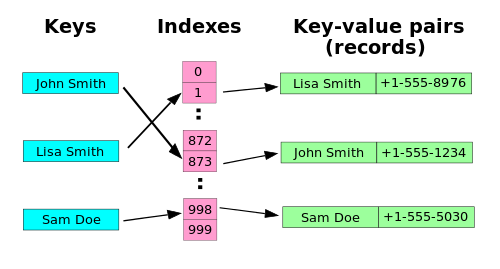
\includegraphics[width=100mm]{HASHTB08.png}
\caption{Κατακερματισμός εγγραφών σε πίνακα κατακερματισμού \cite{wiki_hashtables}}
\label{fig:hashtable1}
\end{figure}

Μια καλή συνάρτηση κατακερματισμού θα πρέπει να κατανέμει τα κλειδιά στα κελιά του πίνακα κατακερματισμού όσο πιο ομοιόμορφα γίνεται και να είναι εύκολο να υπολογιστεί. Επίσης, είναι επιθυμητό το παραγόμενο αποτέλεσμα από τη συνάρτηση κατακερματισμού να εξαρτάται από το κλειδί στο σύνολό του.

Στον κώδικα που ακολουθεί παρουσιάζονται τέσσερις συναρτήσεις κατακερματισμού κάθε μία από τις οποίες δέχεται ένα λεκτικό και επιστρέφει έναν ακέραιο αριθμό. Στις συναρτήσεις hash2 και hash3 γίνεται χρήση τελεστών που εφαρμόζονται σε δυαδικές τιμές (bitwise operators). Ειδικότερα χρησιμοποιούνται οι τελεστές $<<$ (αριστερή ολίσθηση), $>>$ (δεξιά ολίσθηση) και $\hat{}$ (xor - αποκλειστικό ή).

\lstinputlisting[caption = Διάφορες συναρτήσεις κατακερματισμού (hashes.cpp)]{lab07/hashes.cpp}

\lstinputlisting[caption = Παραδείγματα κλήσεων συναρτήσεων κατακερματισμού (hashes\_ex1.cpp)]{lab07/hashes_ex1.cpp}

\lstinputlisting[style=DOS]{lab07/hashes_ex1.out}


Οι πίνακες κατακερματισμού είναι ιδιαίτερα κατάλληλοι για εφαρμογές στις οποίες πραγματοποιούνται συχνές αναζητήσεις εγγραφών με δεδομένες τιμές κλειδιών. Οι βασικές λειτουργίες που υποστηρίζονται σε έναν πίνακα κατακερματισμού είναι η εισαγωγή (insert), η αναζήτηση (get) και η διαγραφή (erase). Και οι τρεις αυτές λειτουργίες παρέχονται σε χρόνο $O(1)$ κατά μέσο όρο προσφέροντας ταχύτερη υλοποίηση σε σχέση με άλλες υλοποιήσεις όπως για παράδειγμα τα ισοζυγισμένα δυαδικά δένδρα αναζήτησης που παρέχουν τις ίδιες λειτουργίες σε χρόνο $O(log n)$. 

Ωστόσο, οι πίνακες κατακερματισμού έχουν και μειονεκτήματα καθώς είναι δύσκολο να επεκταθούν από τη στιγμή που έχουν δημιουργηθεί και μετά. Επίσης, η απόδοση των πινάκων κατακερματισμού υποβαθμίζεται καθώς οι θέσεις τους γεμίζουν με στοιχεία. Συνεπώς, εφόσον ο προγραμματιστής προχωρήσει στη δική του υλοποίηση ενός πίνακα κατακερματισμού είτε θα πρέπει να γνωρίζει εκ των προτέρων το πλήθος των στοιχείων που πρόκειται να αποθηκευτούν είτε όταν αυτό απαιτηθεί να υπάρχει πρόβλεψη έτσι ώστε τα δεδομένα να μεταφέρονται σε μεγαλύτερο πίνακα κατακερματισμού.

Στις περισσότερες εφαρμογές υπάρχουν πολύ περισσότερα πιθανά κλειδιά εγγραφών από ότι θέσεις στο πίνακα κατακερματισμού. Αν για δύο ή περισσότερα κλειδιά η εφαρμογή της συνάρτησης κατακερματισμού επιστρέφει το ίδιο αποτέλεσμα τότε λέμε ότι συμβαίνει σύγκρουση (collision) η οποία θα πρέπει να διευθετηθεί με κάποιο τρόπο. Ο ακόλουθος κώδικας μετρά το πλήθος των συγκρούσεων που συμβαίνουν καθώς δημιουργούνται hashes για ένα σύνολο 2.000 κλειδιών αλφαριθμητικού τύπου.


\lstinputlisting[caption = Δημιουργία τυχαίων λεκτικών (random\_strings.cpp)]{lab07/random_strings.cpp}

\lstinputlisting[caption = Συγκρούσεις (hashes\_ex2.cpp)]{lab07/hashes_ex2.cpp}

\lstinputlisting[style=DOS]{lab07/hashes_ex2.out}

Γενικότερα, σε έναν πίνακα κατακερματισμού, η εύρεση μιας εγγραφής με κλειδί key είναι μια διαδικασία δύο βημάτων:
\begin{itemize}[noitemsep]
\item Εφαρμογή της συνάρτησης κατακερματισμού στο κλειδί της εγγραφής.
\item Ξεκινώντας από την θέση που υποδεικνύει η συνάρτηση κατακερματισμού στον πίνακα κατακερματισμού, εντοπισμός της εγγραφής που περιέχει το ζητούμενο κλειδί (ενδεχόμενα θα χρειαστεί να εφαρμοστεί κάποιος μηχανισμός διευθέτησης συγκρούσεων). 
\end{itemize}

Οι βασικοί μηχανισμοί επίλυσης των συγκρούσεων είναι η ανοικτή διευθυνσιοδότηση και ο κατακερματισμός με αλυσίδες.

\subsection{Ανοικτή διευθυνσιοδότηση}
Στην ανοικτή διευθυνσιοδότηση (open addressing, closed hashing) όλα τα δεδομένα αποθηκεύονται απευθείας στον πίνακα κατακερματισμού. Αν συμβεί σύγκρουση τότε ελέγχεται αν κάποιο από τα υπόλοιπα κελιά είναι διαθέσιμο και η εγγραφή τοποθετείται εκεί. Συνεπώς, θα πρέπει το μέγεθος του hashtable να είναι μεγαλύτερο ή ίσο από το πλήθος των στοιχείων που πρόκειται να αποθηκευτούν σε αυτό. Θα πρέπει να σημειωθεί ότι η απόδοση της ανοικτής διευθυνσιοδότησης μειώνεται κατακόρυφα σε περίπτωση που το hashtable είναι σχεδόν γεμάτο. 

Αν το πλήθος των κελιών είναι $m$ και το πλήθος των εγγραφών είναι $n$ τότε το πηλίκο $a=\frac{n}{m}$ που ονομάζεται παράγοντας φόρτωσης (load factor) καθορίζει σημαντικά την απόδοση του hashtable. Ο παράγοντας φόρτωσης στην περίπτωση της ανοικτής διευθυνσιοδότησης δεν μπορεί να είναι μεγαλύτερος της μονάδας.

Υπάρχουν πολλές παραλλαγές της ανοικτής διευθυνσιοδότησης που σχετίζονται με τον τρόπο που σε περίπτωση σύγκρουσης επιλέγεται το επόμενο κελί που εξετάζεται αν είναι ελεύθερο προκειμένου να τοποθετηθούν εκεί τα δεδομένα της εγγραφής. Αν εξετάζεται το αμέσως επόμενο στη σειρά κελί και μέχρι να βρεθεί το πρώτο διαθέσιμο, ξεκινώντας από την αρχή του πίνακα αν βρεθεί στο τέλος, τότε η μέθοδος ονομάζεται γραμμική ανίχνευση (linear probing). Άλλες διαδεδομένες μέθοδοι είναι η τετραγωνική ανίχνευση (quadratic probing) και ο διπλός κατακερματισμός (double hashing) \cite{visualalgo_hashtables}.

\begin{figure}[ht!]
\centering
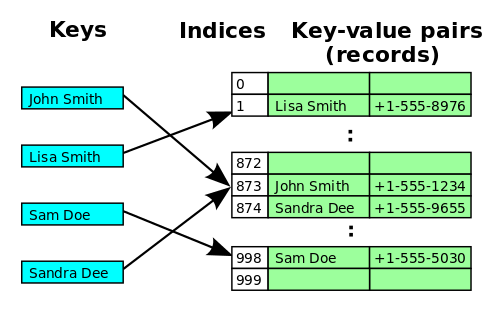
\includegraphics[width=100mm]{HASHTB12.png}
\caption{Κατακερματισμός εγγραφών με ανοικτή διευθυνσιοδότηση και γραμμική ανίχνευση \cite{wiki_hashtables}}
\label{fig:hashtable2}
\end{figure}

Στη συνέχεια ακολουθεί μια υλοποίηση ενός πίνακα κατακερματισμού με ανοικτή διευθυνσιοδότηση και γραμμική ανίχνευση. Στον πίνακα κατακερματισμού τοποθετούνται εγγραφές με κλειδιά και τιμές αλφαριθμητικού τύπου. 

\lstinputlisting[label={lst:open_addressing},caption={Ανοικτή διευθυνσιοδότηση (open\_addressing.cpp)}]{lab07/open_addressing.cpp}

\lstinputlisting[style=DOS]{lab07/open_addressing.out}

\subsection{Κατακερματισμός με αλυσίδες}
Στον κατακερματισμό με αλυσίδες (separate chaining) οι εγγραφές αποθηκεύονται σε συνδεδεμένες λίστες κάθε μια από τις οποίες είναι προσαρτημένες στα κελιά ενός hashtable. Συνεπώς, η απόδοση των αναζητήσεων εξαρτάται από τα μήκη των συνδεδεμένων λιστών. Αν η συνάρτηση κατακερματισμού κατανέμει τα $n$ κλειδιά ανάμεσα στα $m$ κελιά ομοιόμορφα τότε κάθε λίστα θα έχει μήκος $\frac{n}{m}$. O παράγοντας φόρτωσης, $a=\frac{n}{m}$, στον κατακερματισμό με αλυσίδες δεν θα πρέπει να απέχει πολύ από την μονάδα. Πολύ μικρό load factor σημαίνει ότι υπάρχουν πολλές κενές λίστες και συνεπώς δεν γίνεται αποδοτική χρήση του χώρου ενώ μεγάλο load factor σημαίνει μακριές συνδεδεμένες λίστες και μεγαλύτεροι χρόνοι αναζήτησης. 

\begin{figure}[ht!]
\centering
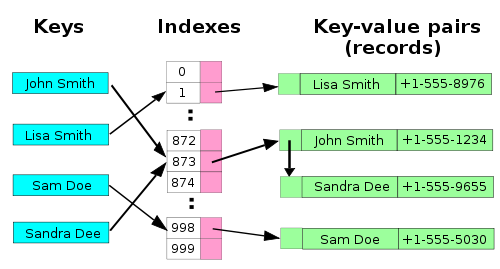
\includegraphics[width=100mm]{HASHTB32.png}
\caption{Κατακερματισμός εγγραφών με αλυσίδες \cite{wiki_hashtables}}
\label{fig:hashtable3}
\end{figure}

Στη συνέχεια ακολουθεί μια υλοποίηση ενός πίνακα κατακερματισμού με κατακερματισμό με αλυσίδες. Για τις συνδεδεμένες λίστες χρησιμοποιείται η λίστα std::list.

\lstinputlisting[caption = Κατακερματισμός με αλυσίδες (separate\_chaining.cpp)]{lab07/separate_chaining.cpp}

\lstinputlisting[style=DOS]{lab07/separate_chaining.out}

Περισσότερες πληροφορίες σχετικά με τον κατακερματισμό και την υλοποίηση πινάκων κατακερματισμού μπορούν να βρεθούν στις αναφορές \cite{pumpkin_hashtables}, \cite{hackerearth_hashtables}.

\section{Κατακερματισμός με την STL}
Η STL διαθέτει την κλάση std::hash που μπορεί να χρησιμοποιηθεί για την επιστροφή hash τιμών για διάφορους τύπους δεδομένων. Στον ακόλουθο κώδικα παρουσιάζεται η χρήση της std::hash.

\lstinputlisting[caption = Παράδειγμα χρήσης της std::hash (stl\_hash.cpp)]{lab07/stl_hash.cpp}

\lstinputlisting[style=DOS]{lab07/stl_hash.out}
 

Επιπλέον, η STL υποστηρίζει δύο βασικές δομές κατακερματισμού το std::unordered\_set και το std::unordered\_map. Το std::unordered\_set υλοποιείται ως ένας πίνακας κατακερματισμού και μπορεί να περιέχει τιμές (κλειδιά) οποιουδήποτε τύπου οι οποίες γίνονται hash σε διάφορες θέσεις του πίνακα κατακερματισμού. Κατά μέσο όρο, οι λειτουργίες σε ένα std::unordered\_set (εύρεση, εισαγωγή και διαγραφή κλειδιού) πραγματοποιούνται σε σταθερό χρόνο O(1). Ένα std::unordered\_set δεν περιέχει διπλότυπα, ενώ αν υπάρχει αυτή η ανάγκη τότε μπορεί να χρησιμοποιηθεί το std::unordered\_multiset. 

Στον κώδικα που ακολουθεί οι χαρακτήρες ενός λεκτικού εισάγονται ένας προς ένας σε ένα std::unordered\_set έτσι ώστε να υπολογιστεί το πλήθος των διακριτών χαρακτήρων ενός λεκτικού.

\lstinputlisting[caption = Παράδειγμα χρήσης του std::unordered\_set (stl\_unordered\_set.cpp)]{lab07/stl_unordered_set.cpp}

\lstinputlisting[style=DOS]{lab07/stl_unordered_set.out}

To std::unordered\_map αποθηκεύει ζεύγη (κλειδί-τιμή). Το κλειδί αναγνωριζει με μοναδικό τρόπο το κάθε ζεύγος και γίνεται hash σε συγκεκριμένη θέση του πίνακα κατακερματισμού. Όπως και στο std::unordered\_set. κατά μέσο όρο, οι λειτουργίες σε ένα std::unordered\_map πραγματοποιούνται σε σταθερό χρόνο O(1). Η ανάθεση τιμής σε κλειδί μπορεί να γίνει με τους τελεστές = και [], ενώ το πέρασμα από τις τιμές ενός std::unordered\_map μπορεί να γίνει με  iterator ή με range for.
 
\lstinputlisting[caption = Παράδειγμα χρήσης του std::unordered\_map (stl\_unordered\_map.cpp)]{lab07/stl_unordered_map.cpp}

\lstinputlisting[style=DOS]{lab07/stl_unordered_map.out}

%\section{Κατακερματισμός και κρυπτογράφηση}
%
%\section{Bloom filters}
%A Bloom filter is a space-efficient probabilistic data structure, conceived by Burton Howard Bloom in 1970, that is used to test whether an element is a member of a set. False positive matches are possible, but false negatives are not – in other words, a query returns either "possibly in set" or "definitely not in set". Elements can be added to the set, but not removed (though this can be addressed with a "counting" filter); the more elements that are added to the set, the larger the probability of false positives.

\section{Παραδείγματα}

\subsection{Παράδειγμα 1}
Έστω μια επιχείρηση η οποία επιθυμεί να αποθηκεύσει τα στοιχεία των υπαλλήλων της (όνομα, διεύθυνση) σε μια δομή έτσι ώστε με βάση το όνομα του υπαλλήλου να επιτυγχάνει τη γρήγορη ανάκληση των υπόλοιπων στοιχείων των υπαλλήλων. Στη συνέχεια παρουσιάζεται η υλοποίηση ενός πίνακα κατακερματισμού στον οποίο κλειδί θεωρείται το όνομα του υπαλλήλου και η επίλυση των συγκρούσεων πραγματοποιείται με ανοικτή διευθυνσιοδότηση (open addressing) και γραμμική ανίχνευση (linear probing). Καθώς δεν υπάρχει η ανάγκη διαγραφής τιμών από τον πίνακα κατακερματισμού παρουσιάζεται μια απλούστερη υλοποίηση σε σχέση με αυτή που παρουσιάστηκε στον κώδικα \ref{lst:open_addressing}. Ο πίνακας κατακερματισμού μπορεί να δεχθεί το πολύ 100.000 εγγραφές υπαλλήλων. Στο παράδειγμα χρονομετρείται η εκτέλεση για 20.000, 30.000 και 80.000 υπαλλήλους. Παρατηρείται ότι λόγω των συγκρούσεων καθώς ο συντελεστής φόρτωσης του πίνακα κατακερματισμού αυξάνεται η απόδοση της δομής υποβαθμίζεται.

\lstinputlisting[caption = Yλοποίηση πίνακα κατακερματισμού για γρήγορη αποθήκευση και αναζήτηση εγγραφών (lab07\_ex1.cpp)]{lab07/lab07_ex1.cpp}

\lstinputlisting[style=DOS]{lab07/lab07_ex1.out}

\subsection{Παράδειγμα 2}
Στο παράδειγμα αυτό παρουσιάζεται η λύση του ίδιου προβλήματος με το παράδειγμα 1 με τη διαφορά ότι πλέον χρησιμοποιείται η δομή std::unordered\_map της STL.

\lstinputlisting[caption = Γρήγορη αποθήκευση και αναζήτηση εγγραφών με τη χρήση της std::unordered\_map (lab07\_ex2.cpp)]{lab07/lab07_ex2.cpp}

\lstinputlisting[style=DOS]{lab07/lab07_ex2.out}

\subsection{Παράδειγμα 3}
Στο παράδειγμα αυτό εξετάζονται τέσσερις διαφορετικοί τρόποι με τους οποίους ελέγχεται για ένα μεγάλο πλήθος τιμών (5.000.000) πόσες από αυτές περιέχονται σε ένα δεδομένο σύνολο 1.000 τιμών. Οι τιμές είναι ακέραιες και επιλέγονται με τυχαίο τρόπο στο διάστημα [0,100.000]. Ο χρόνος που απαιτεί η κάθε προσέγγιση χρονομετρείται.
\begin{itemize}[noitemsep]
\item Η πρώτη προσέγγιση (scenario1) χρησιμοποιεί ένα vector για να αποθηκεύσει το σύνολο των 1.000 τυχαίων ακεραίων τιμών και αναζητά σειριακά κάθε τιμή στο vector. 
\item Η δεύτερη προσέγγιση (scenario2) χρησιμοποιεί επίσης ένα vector για να αποθηκεύσει το σύνολο των 1.000 τυχαίων ακεραίων τιμών, τις ταξινομεί και αναζητά κάθε τιμή στο ταξινομημένο vector. 
\item Η τρίτη προσέγγιση (scenario3) αποθηκεύει τις 1.000 τυχαίες ακεραίες τιμές σε ένα std::set (υλοποιείται στην STL ως δυαδικό δένδρο αναζήτησης) και αναζητά κάθε τιμή σε αυτό. 
\item Η τέταρτη προσέγγιση (scenario4) αποθηκεύει τις 1.000 τυχαίες ακεραίες τιμές σε ένα std::unordered\_set (υλοποιείται στην STL ως πίνακας κατακερματισμού) και αναζητά κάθε τιμή σε αυτό.
%\item Η πέμπτη προσέγγιση (scenario5) υλοποιεί ένα Bloom filter που χρησιμοποιεί ως βασική δομή ένα σύνολο δυαδικών ψηφίων με μέγεθος 10.001. 
\end{itemize}

\lstinputlisting[caption = Έλεγχος ύπαρξης τιμών σε ένα σύνολο τιμών (lab07\_ex3.cpp)]{lab07/lab07_ex3.cpp}

\lstinputlisting[style=DOS]{lab07/lab07_ex3.out}

\section{Ασκήσεις}
\begin{enumerate}
\item Γράψτε μια συνάρτηση που να δέχεται έναν πίνακα ακεραίων Α και έναν ακέραιο αριθμό sum και να βρίσκει το πλήθος από όλα τα ζεύγη τιμών του Α που το άθροισμά τους είναι ίσο με sum.
\item Γράψτε ένα πρόγραμμα που για ένα λεκτικό που θα δέχεται ως είσοδο, να επιστρέφει το χαρακτήρα (γράμματα κεφαλαία, γράμματα πεζά, ψηφία, σύμβολα) που εμφανίζεται περισσότερες φορές καθώς και πόσες φορές εμφανίζεται στο λεκτικό.
\item Γράψτε μια συνάρτηση που να δέχεται έναν πίνακα ακεραίων Α και έναν ακέραιο αριθμό Κ και να βρίσκει τη μεγαλύτερη σε μήκος υποακολουθία στοιχείων του Α που έχει άθροισμα ίσο με Κ.
\item Γράψτε ένα πρόγραμμα που να δέχεται μια λέξη και να βρίσκει γρήγορα όλες τις άλλες έγκυρες λέξεις που είναι αναγραμματισμοί της λέξης που δόθηκε. Θεωρείστε ότι έχετε δεδομένο ένα αρχείο κειμένου με όλες τις έγκυρες λέξεις (words.txt), μια ανά γραμμή.
\end{enumerate}

\begin{thebibliography}{9}
\bibitem{wiki_hashtables}
Wikibooks, Data Structures - Hash Tables, \href{https://en.wikibooks.org/wiki/Data_Structures/Hash_Tables}{https://en.wikibooks.org/wiki/Data\_Structures/Hash\_Tables}

\bibitem{pumpkin_hashtables}
C++ tutorial: Intro to Hash Tables,
\href{https://pumpkinprogrammerdotcom4.wordpress.com/2014/06/21/c-tutorial-intro-to-hash-tables/}{https://pumpkinprogrammerdotcom4.wordpress.com/2014/06/21/c-tutorial-intro-to-hash-tables/}

\bibitem{hackerearth_hashtables}
HackerEarth, Basics of Hash Tables, \href{https://www.hackerearth.com/practice/data-structures/hash-tables/basics-of-hash-tables/tutorial/}{https://www.hackerearth.com/practice/data-structures/hash-tables/basics-of-hash-tables/tutorial/}

\bibitem{visualalgo_hashtables}
VisualAlgo.net Open Addressing (LP, QP, DH) and Separate Chaining Visualization, \href{https://visualgo.net/en/hashtable}{https://visualgo.net/en/hashtable}

\end{thebibliography}

